% !TeX root = RJwrapper.tex
\title{Partitioned Local Depth (PaLD) Clustering Analyses in R}
\author{by Lucy D'Agostino McGowan, Katherine Moore, and Kenneth Berenhaut}

\maketitle

\abstract{%
An abstract of less than 150 words.
}

\hypertarget{introduction}{%
\subsection{Introduction}\label{introduction}}

\begin{itemize}
\tightlist
\item
  Describe PaLD (Ken \& Kate?) \citep{berenhaut2022social}
\end{itemize}

We present a new package, \CRANpkg{pald}, for calculating partitioned
local depth (PaLD) probabilities, implementing clustering analyses, and
creating data visualizations to represent the clusters. This paper will
describe how to use the package as well as walk through two examples.

\hypertarget{pald}{%
\subsection{pald}\label{pald}}

The main functions in \CRANpkg{pald} package can be split into 3
categories:

\begin{enumerate}
\def\labelenumi{\arabic{enumi}.}
\tightlist
\item
  Helper functions to organize data into the correct format, into
  distance matrices and then cohesion matrices
\item
  Functions that convert a cohesion matrix into a variety of useful
  formats, including partitioned local depths, clusters, and graphs
\item
  Plotting functions
\end{enumerate}

In addition, the package provides a number of pertinent example data
sets commonly used to demonstrate cluster algorithms, including a
synthetic data set of two-dimensional points created by
\citet{gionis1clustering} to demonstrate clustering aggregation,
clustering data generated from the scikit-learn Python package
\citep{pedregosa2011scikit}, data describing cognate relationships
between words across 87 Indo-European languages \citep{dyen92}, data
compiled by \cite{tissue} of tissue gene expressions, and three example
data sets generated for the \citet{berenhaut2022social} paper.

While it is not a necessity, the \CRANpkg{pald} package is designed to
function well with the pipe operator, \texttt{\textbar{}\textgreater{}}.
This functionality will be demonstrated below.

\hypertarget{creating-the-cohesion-matrix}{%
\subsubsection{Creating the cohesion
matrix}\label{creating-the-cohesion-matrix}}

For demonstration purposes, below is a sample data frame with two
variables, \texttt{x1} and \texttt{x2}. The methods put forth here work
on data frames with higher dimensions, as described in the
\textbf{Examples} section; we are simply choosing a small data frame
here for demonstration purposes.

\begin{Schunk}
\begin{Sinput}
library(pald)
df <- data.frame(
  x1 = c(6, 8, 11, 16, 4, 14),
  x2 = c(5, 4, 13, 7, 6, 10)
)
rownames(df) <- c("A", "B", "C", "D", "E", "F")
\end{Sinput}
\end{Schunk}

The first step needed to calculate the partitioned local depths is to
construct a \emph{distance matrix}. If the data are already in this
form, the user can skip to the next step. The \texttt{dist()} function
converts an input data frame into a distance matrix, as demonstrated
below.

\begin{Schunk}
\begin{Sinput}
d <- dist(df)
\end{Sinput}
\end{Schunk}

This will create a \texttt{dist} object. If converted to a matrix, this
will be a \(n\times n\) distance matrix, where \(n\) corresponds to the
number of observations in the original data frame, in this example
\(n = 6\).

This dist object, or equivalently a distance matrix, can then be passed
to the \texttt{cohesion\_matrix()} function in order to calculate the
pairwise cohesion values. Cohesion is an interpretable probability that
reflects the strength of alignment of two points. Again, if the user
begins with a distance matrix, they can skip the first step and simply
input the distance matrix into this function.

\begin{Schunk}
\begin{Sinput}
d <- dist(df)
cohesion_matrix(d)
\end{Sinput}
\begin{Soutput}
#>           A         B         C         D         E         F
#> A 0.2333333 0.1666667 0.0000000 0.0000000 0.1666667 0.0000000
#> B 0.1333333 0.2333333 0.0000000 0.0000000 0.1000000 0.0000000
#> C 0.0000000 0.0000000 0.2333333 0.1000000 0.0000000 0.1000000
#> D 0.0000000 0.0000000 0.1000000 0.2666667 0.0000000 0.1666667
#> E 0.1333333 0.1000000 0.0000000 0.0000000 0.2333333 0.0000000
#> F 0.0000000 0.0000000 0.1000000 0.1666667 0.0000000 0.2666667
#> attr(,"class")
#> [1] "cohesion_matrix" "matrix"          "array"
\end{Soutput}
\end{Schunk}

Equivalently, the user can use the native pipe
\texttt{\textbar{}\textgreater{}} as follows.

\begin{Schunk}
\begin{Sinput}
df |>
  dist() |>
  cohesion_matrix()
\end{Sinput}
\begin{Soutput}
#>           A         B         C         D         E         F
#> A 0.2333333 0.1666667 0.0000000 0.0000000 0.1666667 0.0000000
#> B 0.1333333 0.2333333 0.0000000 0.0000000 0.1000000 0.0000000
#> C 0.0000000 0.0000000 0.2333333 0.1000000 0.0000000 0.1000000
#> D 0.0000000 0.0000000 0.1000000 0.2666667 0.0000000 0.1666667
#> E 0.1333333 0.1000000 0.0000000 0.0000000 0.2333333 0.0000000
#> F 0.0000000 0.0000000 0.1000000 0.1666667 0.0000000 0.2666667
#> attr(,"class")
#> [1] "cohesion_matrix" "matrix"          "array"
\end{Soutput}
\end{Schunk}

The \emph{cohesion matrix} output by the \texttt{cohesion\_matrix()} is
the main input for the majority of the remaining functions.

\hypertarget{functions-that-convert-a-cohesion-matrix-into-useful-formats}{%
\subsubsection{Functions that convert a cohesion matrix into useful
formats}\label{functions-that-convert-a-cohesion-matrix-into-useful-formats}}

From the \emph{cohesion matrix}, a variety of useful quantities can be
calculated. Below, we create a cohesion matrix using the functions
described in the previous section.

\begin{Schunk}
\begin{Sinput}
df |>
  dist() |>
  cohesion_matrix() -> cohesion
\end{Sinput}
\end{Schunk}

To calculate the \emph{clusters} that each point will fall into, we can
use the \texttt{community\_clusters()} function. This will output a data
frame with two columns, the first will correspond to the \texttt{point},
as identified by the row name of the original input data frame,
\texttt{df}, the second will identify the \texttt{cluster} that each
point belongs to.

\begin{Schunk}
\begin{Sinput}
community_clusters(cohesion)
\end{Sinput}
\begin{Soutput}
#>   point cluster
#> A     A       1
#> B     B       1
#> C     C       2
#> D     D       3
#> E     E       1
#> F     F       3
\end{Soutput}
\end{Schunk}

In this example, three clusters are identified with these six points.
Points \texttt{A}, \texttt{B}, and \texttt{E} fall into cluster 1. Point
\texttt{C} is in cluster 2 and points \texttt{D} and \texttt{F} fall
into cluster 3.

The \texttt{local\_depths()} function calculates the \emph{depths} of
each point, outputting a vector of local depths. Local depth is an
interpretable probability which reflects aspects of relative position
and centrality via distance comparisons (i.e., \(d(z, x) < d(z, y)\)).

\begin{Schunk}
\begin{Sinput}
local_depths(cohesion)
\end{Sinput}
\begin{Soutput}
#>         A         B         C         D         E         F 
#> 0.5666667 0.4666667 0.4333333 0.5333333 0.4666667 0.5333333
\end{Soutput}
\end{Schunk}

In this case, the deepest point is \texttt{A}.

The \texttt{strong\_threshold()} function will calculate the cohesion
threshold for strong ties. This is equal to half the average of the
diagonal cohesion matrix. This is a threshold that may be used to
distinguish between strong and weak ties.

\begin{Schunk}
\begin{Sinput}
strong_threshold(cohesion)
\end{Sinput}
\begin{Soutput}
#> [1] 0.1222222
\end{Soutput}
\end{Schunk}

In this case, the threshold is \texttt{0.12}.

The \texttt{any\_isolated()} function will check whether there are any
isolated points that will inadvertently be dropped by a graph.

\begin{Schunk}
\begin{Sinput}
any_isolated(cohesion)
\end{Sinput}
\end{Schunk}

Here, there are no isolated points.

The function \texttt{cohesion\_strong()} will update the cohesion matrix
to set all weak ties to zero (via the \texttt{strong\_threshold()}
function). Optionally, the matrix will also be symmetrized, with the
default parameter \texttt{symmetric\ =\ TRUE}.

\begin{Schunk}
\begin{Sinput}
cohesion_strong(cohesion)
\end{Sinput}
\begin{Soutput}
#>           A         B         C         D         E         F
#> A 0.2333333 0.1333333 0.0000000 0.0000000 0.1333333 0.0000000
#> B 0.1333333 0.2333333 0.0000000 0.0000000 0.0000000 0.0000000
#> C 0.0000000 0.0000000 0.2333333 0.0000000 0.0000000 0.0000000
#> D 0.0000000 0.0000000 0.0000000 0.2666667 0.0000000 0.1666667
#> E 0.1333333 0.0000000 0.0000000 0.0000000 0.2333333 0.0000000
#> F 0.0000000 0.0000000 0.0000000 0.1666667 0.0000000 0.2666667
#> attr(,"class")
#> [1] "cohesion_matrix" "matrix"          "array"
\end{Soutput}
\end{Schunk}

Finally, the \texttt{community\_graphs()} function takes the cohesion
matrix and creates \CRANpkg{igraph} objects, graphs that describes the
relationship between the points. This function will output a list of
three objects:

\begin{itemize}
\tightlist
\item
  \texttt{G}: the weighted (community) graph whose edge weights are
  mutual cohesion
\item
  \texttt{G\_strong}: the weighted (community) graph consisting of edges
  for which mutual cohesion is greater than the threshold for strong
  ties
\item
  \texttt{layout}: the graph layout, using the Fruchterman Reingold (FR)
  force-directed graph drawing for the graph \texttt{G}
\end{itemize}

\begin{Schunk}
\begin{Sinput}
graphs <- community_graphs(cohesion)
graphs[["G_strong"]]
\end{Sinput}
\begin{Soutput}
#> IGRAPH dcdcffa UNW- 6 3 -- 
#> + attr: name (v/c), weight (e/n)
#> + edges from dcdcffa (vertex names):
#> [1] A--B A--E D--F
\end{Soutput}
\end{Schunk}

Here we see that there are three connected components, points \texttt{A}
and \texttt{B}, and \texttt{A} and \texttt{E} which form the first
cluster, and points \texttt{D} and \texttt{F} which form another.

\hypertarget{plotting-functions}{%
\subsection{Plotting functions}\label{plotting-functions}}

The final category of function is functions for data visualization. We
can begin by visualizing the points in data frame \texttt{df} (Figure
\ref{fig:fig1}). When visualizing these points, it is important to have
a square plot so as to not distort the distances. When using the
\CRANpkg{ggplot2} package for this visualization, you can use the
\texttt{aspect.ratio\ \ =\ 1} argument in the \texttt{theme()} function.
If using the \texttt{plot()} function included in the base library, you
can set the plot area to be a square by using \texttt{par(pty\ =\ "s")}
prior to calling the \texttt{plot()} function, as shown below.

\begin{Schunk}
\begin{Sinput}
library(ggplot2)
ggplot(df, aes(x1, x2)) +
  geom_text(label = rownames(df)) + 
  theme(aspect.ratio = 1)
\end{Sinput}
\begin{figure}
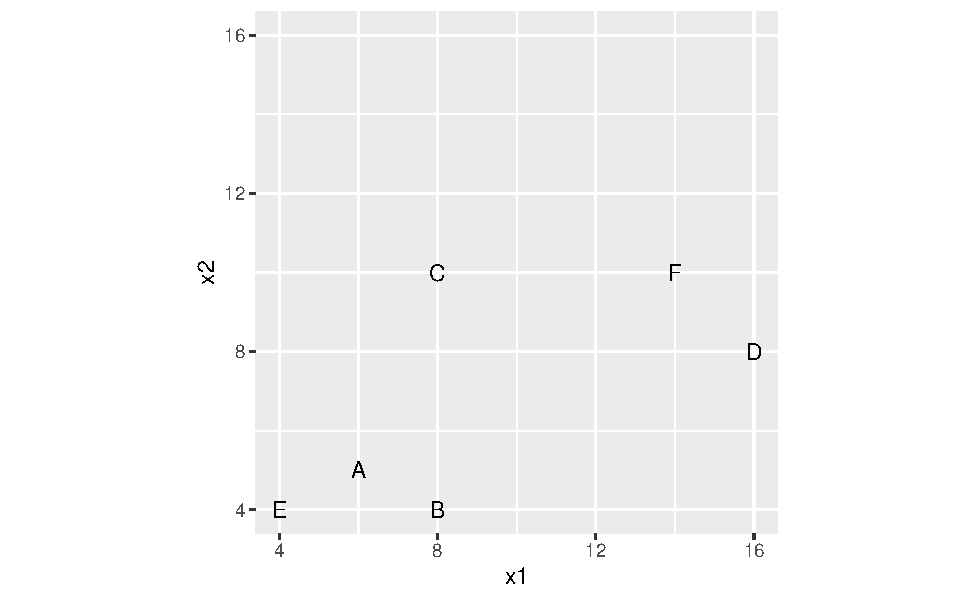
\includegraphics{manuscript_files/figure-latex/fig1-1} \caption[Visualize the points from data frame `df`]{Visualize the points from data frame `df`}\label{fig:fig1}
\end{figure}
\end{Schunk}

We can pass the cohesion matrix to the
\texttt{plot\_community\_graphs()} function to view the relationship
between points (Figure \ref{fig:fig2}).

\begin{Schunk}
\begin{Sinput}
plot_community_graphs(cohesion)
\end{Sinput}
\begin{figure}
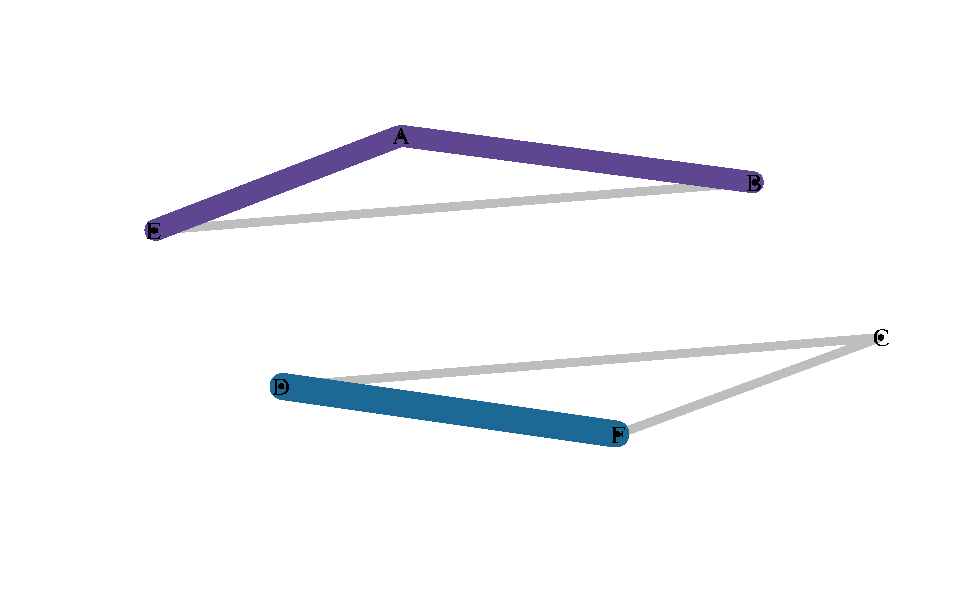
\includegraphics{manuscript_files/figure-latex/fig2-1} \caption[PaLD graph displaying the relationship between the points in data frame `df`]{PaLD graph displaying the relationship between the points in data frame `df`}\label{fig:fig2}
\end{figure}
\end{Schunk}

The \texttt{layout} argument allows the user to pass a matrix to dictate
the layout of the graph. For example, if we wanted the graph to match
the visualization displayed in Figure \ref{fig:fig1}, we can pass
\texttt{as.matrix(df)}, or a matrix of the data frame \texttt{df} to the
\texttt{layout} argument (Figure \ref{fig:fig3}. Notice in the code
below, we set \texttt{par(pty\ =\ "s")} in order to ensure that we have
a square plotting region. Additionally, this
\texttt{plot\_community\_graphs()} function will also permit parameters
that can be passed to the \texttt{plot.igraph()} function. For example,
we can pass arguments to the \texttt{plot.igraph} function via the
\texttt{...}, for example to increase the vertex size and change the
vertex label color, we can specify \texttt{vertex.size\ =\ 15} and
\texttt{vertex.label.color\ =\ "white"}.

\begin{Schunk}
\begin{Sinput}
par(pty = "s")

plot_community_graphs(cohesion, 
                      layout = as.matrix(df),
                      vertex.size = 15,
                      vertex.label.color = "white")
\end{Sinput}
\begin{figure}
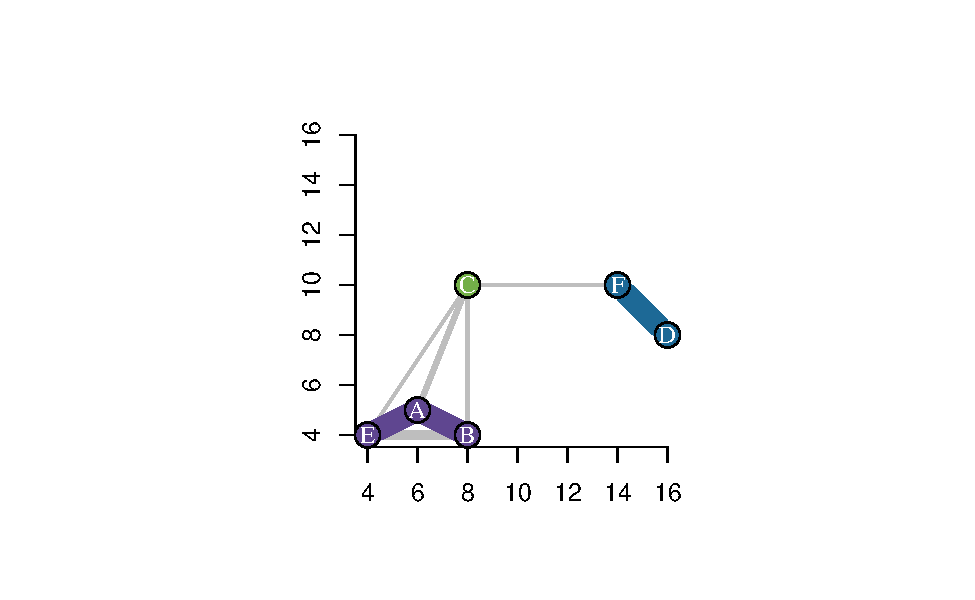
\includegraphics{manuscript_files/figure-latex/fig3-1} \caption[PaLD graph displaying the relationship between the points in data frame `d`, matching the original layout in Figure 1]{PaLD graph displaying the relationship between the points in data frame `d`, matching the original layout in Figure 1}\label{fig:fig3}
\end{figure}
\end{Schunk}

\hypertarget{examples}{%
\subsection{Examples}\label{examples}}

We will demonstrate the utility of the \CRANpkg{pald} package in three
clustering examples.

\hypertarget{clustering-tissue-gene-expression-data}{%
\subsubsection{Clustering tissue gene expression
data}\label{clustering-tissue-gene-expression-data}}

The first example if from a subset of tissue gene expression data from
\citet{zilliox2007gene}, \citet{mccall2011gene}, and
\citet{mccall2014gene}, obtained from the \textbf{tissuesGeneExpression}
bioconductor package \citep{tissue}. A \texttt{dist} object was created
using this data set and is included the \CRANpkg{pald} package in an
object called \texttt{tissue\_dist}.

The \texttt{tissue\_dist} object is a \texttt{dist} object resulting in
a distance matrix with 189 rows and 189 columns.

We can create the cohesion matrix using the \texttt{cohesion\_matrix}
function.

\begin{Schunk}
\begin{Sinput}
tissue_cohesion <- cohesion_matrix(tissue_dist)
\end{Sinput}
\end{Schunk}

The \texttt{community\_clusters()} function can be used to identify the
clusters of each tissue sample. Since the output is a data frame, we can
summarize the clusters using commonly used data analysis techniques. For
demonstration purposes, we will use the \CRANpkg{dplyr} package to
summarize the contribution of clusters.

\begin{Schunk}
\begin{Sinput}
community_clusters(tissue_cohesion) |>
  dplyr::count(cluster, point)
\end{Sinput}
\begin{Soutput}
#>    cluster       point  n
#> 1        1 endometrium 15
#> 2        1      kidney 39
#> 3        2 hippocampus 31
#> 4        3  cerebellum 26
#> 5        4  cerebellum  1
#> 6        5       colon 33
#> 7        6       colon  1
#> 8        7       liver  7
#> 9        8  cerebellum  1
#> 10       9       liver 17
#> 11      10  cerebellum  2
#> 12      11       liver  2
#> 13      12  cerebellum  1
#> 14      13  cerebellum  4
#> 15      14  cerebellum  2
#> 16      15  cerebellum  1
#> 17      16    placenta  2
#> 18      17    placenta  1
#> 19      18    placenta  3
\end{Soutput}
\end{Schunk}

From this, we can glean that cluster one consists of two types of
tissue, the kidney and endometrium. Cluster two is comprised of only the
hippocampus.

We can also display the relationships between tissue samples using the
\texttt{plot\_community\_graphs()} function (Figure \ref{fig:fig4}). For
clarity of the display, we show how to remove the labels using
\texttt{show\_labels\ =\ FALSE}. We will instead color by the labels by
passing these to the \texttt{vertex.color} parameter through the
\texttt{...} to the \texttt{plot.igraph} function. Similarly, we can add
a legend using the \texttt{legend()} function, as you would for a
\CRANpkg{igraph} visualization. Additionally, we use the
\texttt{edge\_width\_factor} and \texttt{emph\_strong} arguments to
adjust the width of the lines between and within PaLD clusters.

\begin{Schunk}
\begin{Sinput}
labels <- rownames(tissue_cohesion)
plot_community_graphs(tissue_cohesion,
                      show_labels = FALSE,
                      vertex.size = 4,
                      vertex.color = as.factor(labels),
                      edge_width_factor = 35,
                      emph_strong = 5) 
legend("topleft", 
       legend = unique(as.factor(labels)), 
       pt.bg = unique(as.factor(labels)),
       col = "black",
       pch = 21)
\end{Sinput}
\end{Schunk}

\begin{Schunk}
\begin{figure}
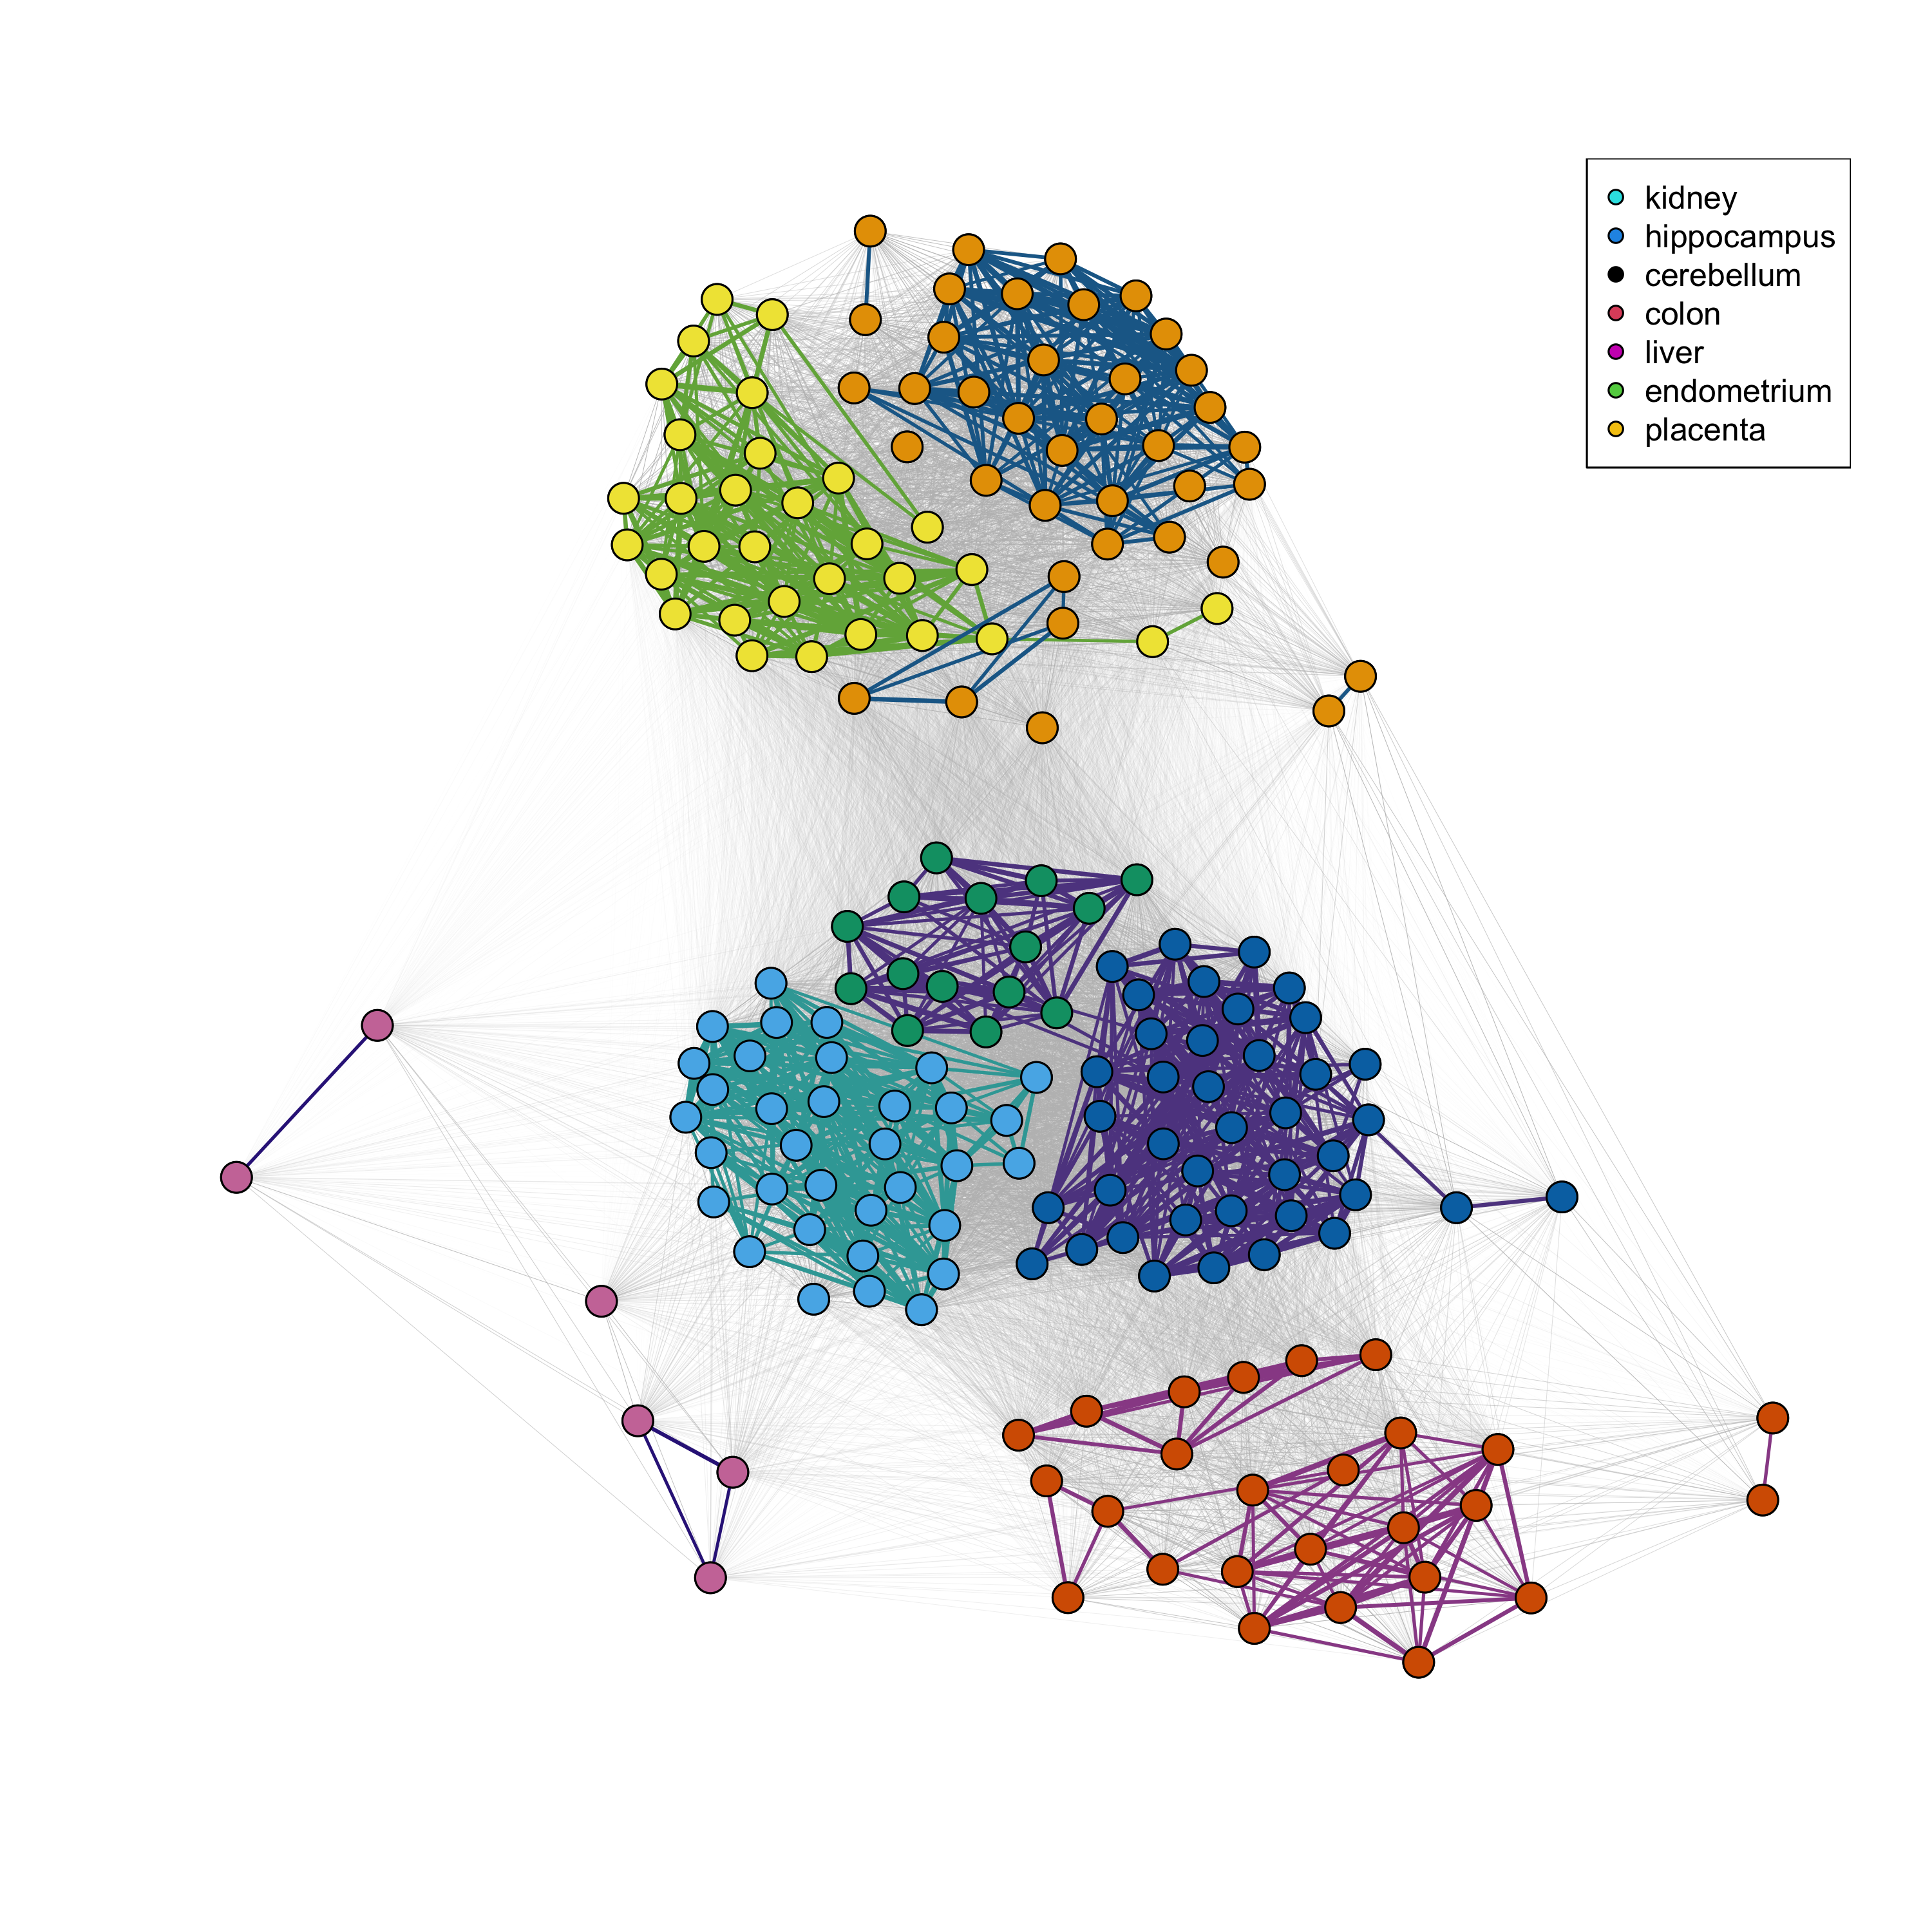
\includegraphics[width=1\linewidth]{fig5} \caption[PaLD clustering of tissue data]{PaLD clustering of tissue data. The line colors indicate the PaLD clusters, the point colors indicate the tissue classification.}\label{fig:fig4}
\end{figure}
\end{Schunk}

\hypertarget{cognate-based-language-families}{%
\subsection{Cognate-based Language
Families}\label{cognate-based-language-families}}

This example performs a PaLD analysis on a data set from \citet{dyen92}
that examines the relationship between 87 Indo-European languages from
the perspective of cognates. A \texttt{dist} object was created from
this data set and included in the \CRANpkg{pald} package in an object
called \texttt{cognate\_dist}.

This example will demonstrate how you can apply functions in the
\CRANpkg{igraph} package to objects output from the \CRANpkg{pald}
package. We can first use the \texttt{cohesion\_matrix()} function to
calculate the cohesion matrix and the \texttt{community\_graphs()}
function to create a list with the weighted community graph, the
weighted community graph with only strong ties included (and all others
set to 0), and the layout. From this, we can extract the graph with only
the strong ties, here called \texttt{cognate\_graph\_strong}.

\begin{Schunk}
\begin{Sinput}
cognate_cohesion <- cohesion_matrix(cognate_dist)
cognate_graphs <- community_graphs(cognate_cohesion)

cognate_graph_strong <- cognate_graphs[["G_strong"]]
\end{Sinput}
\end{Schunk}

We can then use the \texttt{neighbors()} function from the
\CRANpkg{igraph} package to extract the neighbors in this graph. For
example, if we wanted to extract all neighbors where the language is
``French'', we would run the following.

\begin{Schunk}
\begin{Sinput}
french_neighbors <- igraph::neighbors(cognate_graph_strong, "French")
french_neighbors
\end{Sinput}
\begin{Soutput}
#> + 8/87 vertices, named, from 64a847b:
#> [1] Italian         Ladin           Provencal       Walloon        
#> [5] French_Creole_C French_Creole_D Spanish         Catalan
\end{Soutput}
\end{Schunk}

Similarly, we can print the associated neighborhood weights by
subsetting the cohesion matrix.

\begin{Schunk}
\begin{Sinput}
cognate_cohesion["French", french_neighbors]
\end{Sinput}
\begin{Soutput}
#>         Italian           Ladin       Provencal         Walloon French_Creole_C 
#>      0.01997696      0.02094596      0.02871174      0.03258771      0.02406057 
#> French_Creole_D         Spanish         Catalan 
#>      0.02406057      0.01679733      0.01859688
\end{Soutput}
\end{Schunk}

\hypertarget{clustering-generated-data}{%
\subsubsection{Clustering generated
data}\label{clustering-generated-data}}

The \CRANpkg{pald} includes three randomly generated data frames
corresponding to plots from \citet{berenhaut2022social}:

\begin{itemize}
\tightlist
\item
  \texttt{exdata1} is a data set consisting of 8 points to recreate
  Figure 1 in \citet{berenhaut2022social}
\item
  \texttt{exdata2} is a data set consisting of 16 points to recreate
  Figure 2 in \citet{berenhaut2022social}
\item
  \texttt{exdata3} is a data set consisting of 240 points to recreate
  Figure 4D in \citet{berenhaut2022social}
\end{itemize}

Here, we will demonstrate how to use \texttt{exdata3}. These points were
generated from bivariate normal distributions with varying means and
variances. There are eight ``true'' clusters.

We will demonstrate how we can compare PaLD to two clustering methods:
\emph{k}-means and hierarchical clustering. The code below calculates
the cohesion matrix (\texttt{exdata\_cohesion}) as well as the clusters
via PaLD (\texttt{exdata\_pald}), \emph{k}-means
(\texttt{exdata\_kmeans}) and hierarchical clustering
(\texttt{exdata\_hclust}).

\begin{Schunk}
\begin{Sinput}
exdata_cohesion <- exdata3 |>
  dist() |>
  cohesion_matrix()

exdata_pald <- community_clusters(exdata_cohesion)$cluster

exdata_kmeans <- kmeans(exdata3, 8)$cluster

exdata_hclust <- exdata3 |>
  dist() |>
  hclust() |>
  cutree(k = 8) 
\end{Sinput}
\end{Schunk}

We can compare this to the clustering generated by \emph{k}-means and
hierarchical clustering (Figure \ref{fig:fig5}).

\begin{Schunk}
\begin{Sinput}
par(mfrow = c(1, 3), pty = "s")
plot(
  exdata3,
  pch = 16,
  col = pald_colors[exdata_pald],
  xlab = "",
  ylab = "",
  main = "PaLD Clusters"
)
plot(
  exdata3,
  pch = 16,
  col = pald_colors[exdata_kmeans],
  xlab = "",
  ylab = "",
  main = "K-Means Clusters (k = 8)"
)
plot(
  exdata3,
  pch = 16,
  col = pald_colors[exdata_hclust],
  xlab = "",
  ylab = "",
  main = "Hiearchical Clusters (k = 8)"
)
\end{Sinput}
\begin{figure}
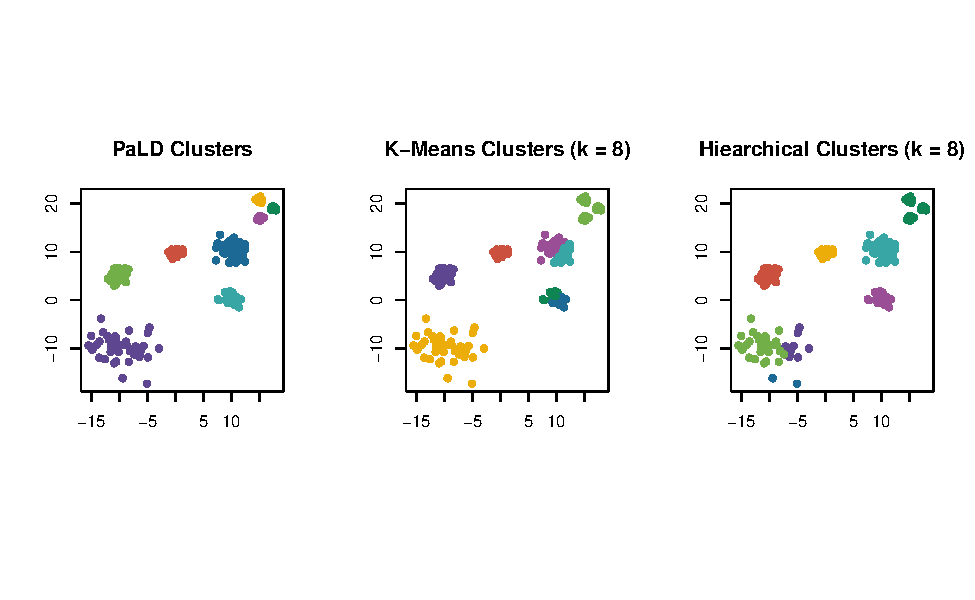
\includegraphics{manuscript_files/figure-latex/fig5-1} \caption[PaLD clustering of randomly generated example data (from Figure 4D from Berenhaut et al]{PaLD clustering of randomly generated example data (from Figure 4D from Berenhaut et al. (2022)) compared to *k*-means and hierarchical clustering with k = 8.}\label{fig:fig5}
\end{figure}
\end{Schunk}

Cohesion is particularly useful when considering data with varying local
density, see discussion in \citep{berenhaut2022social}. Note that the
PaLD algorithm is able to detect the eight natural groups within the
data without the use of any additional inputs (e.g., number of clusters)
nor optimization criteria. Despite providing the ``correct'' number of
clusters (i.e., \(k = 8\)) both \emph{k}-means and hierarchical
clustering did not give the desired result.

The ability of the PaLD algorithm to discern clusters is demonstrated
here.

\hypertarget{summary}{%
\subsection{Summary}\label{summary}}

This paper introduces the \CRANpkg{pald} package, demonstrating it's
utility for providing a parameter-free clustering algorithm that can
easily be applied to any data set.

\bibliography{RJreferences}


\address{%
Lucy D'Agostino McGowan\\
Wake Forest University\\%
Winston-Salem, NC\\ 27106\\
%
%
%
\href{mailto:mcgowald@wfu.edu}{\nolinkurl{mcgowald@wfu.edu}}%
}

\address{%
Katherine Moore\\
Wake Forest Unversity\\%
Winston-Salem, NC\\ 27106\\
%
%
%
\href{mailto:mooreke@wfu.edu}{\nolinkurl{mooreke@wfu.edu}}%
}

\address{%
Kenneth Berenhaut\\
Wake Forest University\\%
Winston-Salem, NC\\ 27106\\
%
%
%
\href{mailto:berenhks@wfu.edu}{\nolinkurl{berenhks@wfu.edu}}%
}
